\subsection{Neuron with Slots}
Each neuron holds a map of slots (weights). Each slot maintains a strength, adaptive threshold, spike-rate EMA, a first-seen flag, and a hit counter up to a saturation limit.

\subsection{Local Learning (bounded reinforcement)}
Strengths are updated with a bounded, non-linear rule scaled by a modulation factor and tempered by inhibition on the layer bus.

\subsection{Adaptive Thresholds (T0+T2)}
On first effective stimulus, T0 sets the threshold just below it. Subsequently, T2 homeostasis nudges the threshold by $\eta\,(\hat r - r^\star)$ where $\hat r$ is the slot's firing EMA.

\subsection{Network Dynamics}
Layers own a lateral bus (inhibition/modulation). Regions orchestrate a two-phase tick: Phase A injects inputs and allows local propagation; Phase B flushes inter-layer tracts once. Output neurons never propagate; instead they accumulate and finalize a frame via EMA.

\begin{figure}[t]
  \centering
  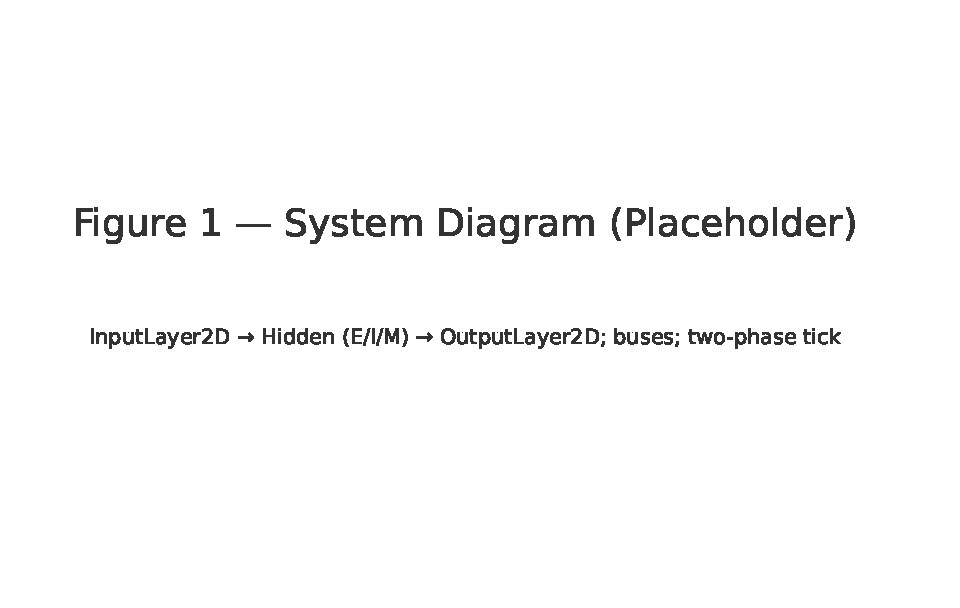
\includegraphics[width=0.95\linewidth]{figures/fig_system.pdf}
  \caption{GrowNet system overview.}
  \label{fig:system}
\end{figure}

\begin{figure}[t]
  \centering
  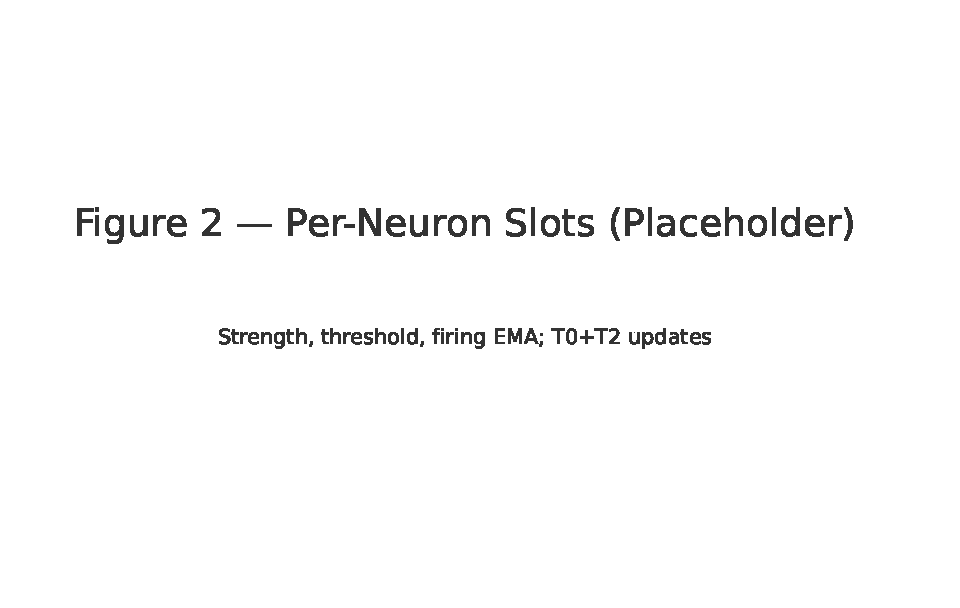
\includegraphics[width=0.85\linewidth]{figures/fig_slot_closeup.pdf}
  \caption{Per-neuron slot close-up with adaptive thresholds (T0+T2).}
  \label{fig:slot}
\end{figure}

\begin{figure}[t]
  \centering
  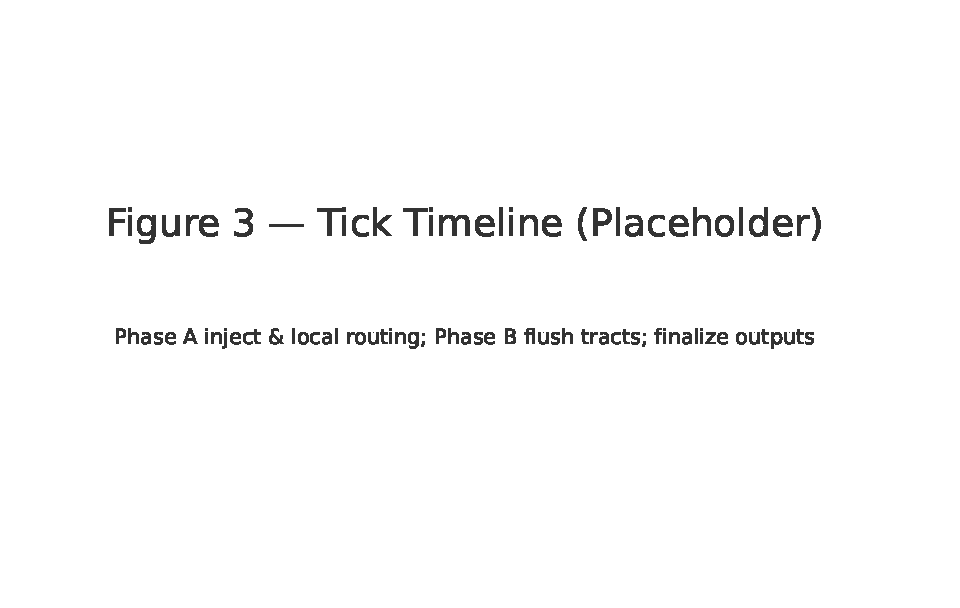
\includegraphics[width=0.95\linewidth]{figures/fig_tick_timeline.pdf}
  \caption{Two-phase tick timeline.}
  \label{fig:timeline}
\end{figure}
